\documentclass[xcolor=pdftex,dvipsnames,table]{beamer}
\usetheme{Darmstadt}
\usepackage{etex}
\providecommand\thispdfpagelabel[1]{}
\usepackage{amsmath}
\usepackage{amssymb}
\usepackage{amsthm}
\usepackage{listings}
\usepackage{graphics}
\usepackage{framed}
\usepackage{etex}
\usepackage[all]{xy}
\usepackage{svg}
\usepackage{xspace,listings,ulem,tikz}
\usepackage[outline]{contour}
\usepackage[absolute,overlay]{textpos}
\usepackage{hhline}
\usepackage{pgffor}
\usepackage[square,sort,comma,numbers]{natbib}
\usepackage{CJKutf8}
\setbeamertemplate{footline}[frame number]
\tikzset{
    onslide/.code args={<#1>#2}{% http://tex.stackexchange.com/a/6155/16595
        \only<#1>{\pgfkeysalso{#2}}
    },
    hideshow/.style args={<#1><#2>#3}{%
        onslide=<#1>{move to},
        onslide=<#2>{#3}
    }
}
\lstset{
         basicstyle=\footnotesize\ttfamily, % Standardschrift
         %numbers=left,               % Ort der Zeilennummern
         numberstyle=\tiny,          % Stil der Zeilennummern
         %stepnumber=2,               % Abstand zwischen den Zeilennummern
         numbersep=5pt,              % Abstand der Nummern zum Text
         tabsize=2,                  % Groesse von Tabs
         extendedchars=true,         %
         breaklines=true,            % Zeilen werden Umgebrochen
         keywordstyle=\color{red},
 %        keywordstyle=[1]\textbf,    % Stil der Keywords
 %        keywordstyle=[2]\textbf,    %
 %        keywordstyle=[3]\textbf,    %
 %        keywordstyle=[4]\textbf,   \sqrt{\sqrt{}} %
         %stringstyle=\color{white}\ttfamily, % Farbe der String
         showspaces=false,           % Leerzeichen anzeigen ?
         showtabs=false,             % Tabs anzeigen ?
         xleftmargin=3pt,
         framexleftmargin=3pt,
         framexrightmargin=1pt,
         framexbottommargin=3pt,
         language=C++,
         %backgroundcolor=\color{lightgray},
         showstringspaces=false      % Leerzeichen in Strings anzeigen ?        
 }

 \usetikzlibrary{arrows}
 \usepackage{caption}
\DeclareCaptionFont{white}{\color{white}}
\DeclareCaptionFormat{listing}{\colorbox[cmyk]{0.43, 0.35, 0.35,0.01}{\parbox{\textwidth}{\hspace{15pt}#1#2#3}}}
\captionsetup[lstlisting]{format=listing,labelfont=white,textfont=white, singlelinecheck=false, margin=0pt, font={bf,footnotesize}}
\beamertemplatenavigationsymbolsempty
\newcommand{\N}{\ensuremath{\mathbb{N}}} 
\newcommand{\R}{\ensuremath{\mathbb{R}}} 
\newcommand{\RR}{\ensuremath{\mathbb{R}}} 
\newcommand{\C}{\ensuremath{\mathbb{C}}} 
\newcommand{\Q}{\ensuremath{\mathbb{Q}}} 
\newcommand{\Z}{\ensuremath{\mathbb{Z}}} 
\newcommand{\D}{\ensuremath{\mathbb{D}}}
\newcommand{\lb}{\mathrm{lb}}
\newcommand{\dy}{\mathrm{dy}}
\newcommand{\cc}{\texttt{C++}\xspace}
\newcommand{\bin}{\mathrm{bin}}
\newcommand{\cl}{\ensuremath{\mathcal{L}}\xspace}
\newcommand{\nc}{\ensuremath{\mathcal{NC}}\xspace}
\newcommand{\fp}{\ensuremath{\mathcal{FP}}\xspace}
\newcommand{\irram}{\texttt{iRRAM}\xspace}
\newcommand{\code}[1]{\texttt{#1}}
\newcommand{\sharpp}{\ensuremath{\#\mathcal P}\xspace}
\newcommand{\sharppu}{\ensuremath{\#{\mathcal P}_1}\xspace}
\newcommand{\sigmas}{\ensuremath{\Sigma^{**}}}
  \newcommand{\complex}{\code{COMPLEX}\xspace}
	\newcommand{\abs}[1]{\left|#1\right|}
  \newcommand{\temp}{\textcolor{red}}
  \newcommand{\seq}{\mathbf}
\newcommand{\fpu}{\ensuremath{\mathcal{FP}_1}\xspace}
\newcommand{\fpt}{\ensuremath{\text{FP}^2}\xspace}
\newcommand{\fpspacet}{\ensuremath{\text{FPSPACE}^2}\xspace}
\newcommand{\sharpt}{\ensuremath{\text{\#P}^2}\xspace}
\newcommand{\pt}{\ensuremath{\text{P}^2}\xspace}
\newcommand{\npt}{\ensuremath{\text{NP}^2}\xspace}
\newcommand{\pspacet}{\ensuremath{\text{PSPACE}^2}\xspace}
\newcommand{\pspace}{\ensuremath{\text{PSPACE}}\xspace}
\DeclareMathOperator{\dom}{\mathrm{dom}}
\newtheorem{conjecture}{Conjecture} 
\newtheorem{representation1}{Representation 1} 
\newtheorem{representation1b}{Representation 1'} 
\newcommand\tab[1][1cm]{\hspace*{#1}}
\newtheorem{representation2}{Representation 2} 
\title[Analytic Functions]{Analytic Functions and Small Complexity Classes}
\author[ H. Thies]{
		Holger Thies \footnote{Joint work with Florian Steinberg}
}
\institute[The University of Tokyo]{
  The University of Tokyo
}
\begin{document}
\setbeamercolor{note}{fg=black,bg=lightgray} 
\date{June 15, 2016}
\frame{
\titlepage
}
\frame{
 \tableofcontents 
}
\section{Type-2 Complexity}
\subsection*{Definition}
\begin{frame}
  \frametitle{Representations}
  A representation for a set $X$ is a partial surjective function $\rho: \Sigma^{**} \to X$.
  \pause
  \vfill
  \begin{minipage}{.37\textwidth}
  \begin{displaymath}
    \xymatrix{
        \Sigma^{**} \ar[r]^F \ar[d]_\alpha & \Sigma^{**} \ar[d]^{\beta} \\
        X \ar[r]_{f}       & Y }
  \end{displaymath} 
  \end{minipage}
  \hfill
  \pause
  \begin{minipage}{.45\textwidth}
    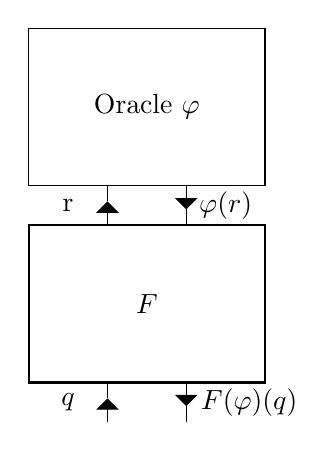
\begin{tikzpicture}
      %x
      \draw (0,0) rectangle (3,-2);
      \node at (1.5,-1) {Oracle $\varphi$};
      \draw (1,-2) -- (1,-2.2);
      \draw[-triangle 90] (1,-2.5) -- (1,-2.2);
      \node at (.5,-2.25) {r};
      \draw[-triangle 90] (2,-2) -- (2,-2.3);
      \draw (2,-2.3) -- (2,-2.5);
      \node at (2.5,-2.25) {$\varphi(r)$};
      %f
      \draw[thick] (0,-2.5) rectangle (3,-4.5);
      \node at (1.5,-3.5) {$F$};
      \draw (1,-4.5) -- (1,-4.7);
      \draw[-triangle 90] (1,-5) -- (1,-4.7);
      \node at (.5,-4.75) {$q$};
      \draw[-triangle 90] (2,-4.5) -- (2,-4.8);
      \draw (2,-4.8) -- (2,-5);
      \node at (2.8,-4.75) {$F(\varphi)(q)$};
      %f(x)
    \end{tikzpicture}
  \end{minipage}
  \end{frame}
\begin{frame}
  \frametitle{Type-2 Complexity Theory}
  \begin{itemize}
  \item Let $\sigmas$ be the set of length-monotone string-functions, i.e. $\abs{x} \leq \abs{y} \Rightarrow \abs{\varphi(x)} \leq \abs{\varphi(y)}$
  \item Consider representation $\varphi : \sigmas \to \sigmas$
  \item Define $\abs{\varphi} : \N \to \N$ by $\abs{\varphi}(\abs{u}) = \abs{\varphi(u)}$
   \item Bound running time by second order polynomials $P(\abs{\varphi})(\abs{x})$
   \item Example: $P(L,n) = 2L(L(L(n)^4+2L(n))+2)+n+10$
   \item  Can define complexity classes \fpt, \sharpt and \fpspacet 
   \item  Can also define complexity classes \pt, \npt and \pspacet by considering functions $\varphi : \sigmas \to (\Sigma^* \to \{0,1\})$
     \item Type-2 classes are easy to seperate
  
  \end{itemize}
\end{frame}
\begin{frame}
  \frametitle{Example}
  Define a $\rho_\R$-name of $x \in \RR$ by
  $\rho_\R(0^n)$ encodes a $d \in \D$ such that $\abs{d-x} \leq 2^{-n} $.
		\begin{figure}
		\centering
    \vfill
		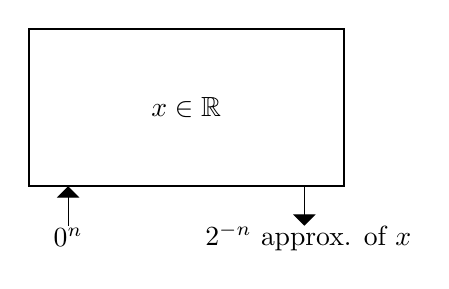
\begin{tikzpicture}
				\path (0,0) rectangle (3.5,-2.7);
			%x
				\draw[thick] (0,0) rectangle (4,-2);
				\node at (2.0,-1) {$x \in \RR$};
				\draw[-triangle 90] (.5,-2.5) -- (.5,-2.0);
				\node at (.5,-2.65) {$0^n$};
				\draw[-triangle 90] (3.5,-2.0) -- (3.5,-2.5);
				\node at (3.55,-2.65) {$2^{-n}$ approx. of $x$};
				%\node<4-> at (2.85,-2.25) {$d_{n,i}$};
				%\node<4-> at (1.5,-1) {$(a_i)$};
				%\draw<4-> (1,-2) -- (1,-2.2);
				%\draw<4->[-triangle 90] (1,-2.5) -- (1,-2.2);
				%\node<4-> at (1.25,-2.25) {$1^i$};
		\end{tikzpicture}
		\end{figure}

  Note, that $(\rho_\R|^{[0,1]}, \rho_\R)$-\fpt equals the polynomial-time computable real functions as defined by Ko.
\end{frame}
\begin{frame}
  \frametitle{Example}
  Define a $\delta_\Box$-name of a function $f \in C[0,1]$ as a pair $<\mu, \phi>$ where $\mu$ encodes the modulus of convergence (in unary) and $\phi$ is such that $\abs{\phi(d, 0^n)-f(d)} \leq 2^{-n}$ for all $d \in \D \cap [0,1]$

		\begin{figure}
		\centering
    \vfill
		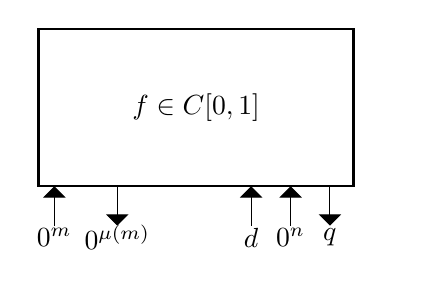
\begin{tikzpicture}
				\path (0,0) rectangle (4.5,-2.7);
			%x
				\draw[thick] (0,0) rectangle (4,-2);
				\node at (2.0,-1) {$f \in C[0,1]$};
				\draw[-triangle 90] (.2,-2.5) -- (.2,-2.0);
				\node at (.2,-2.65) {$0^m$};
				\draw[-triangle 90] (1.0,-2.0) -- (1.0,-2.5);
				\node at (1.0,-2.65) {$0^{\mu(m)}$};
				\draw[-triangle 90] (2.7,-2.5) -- (2.7,-2.0);
				\node at (2.7,-2.65) {$d$};
				\draw[-triangle 90] (3.2,-2.5) -- (3.2,-2.0);
				\node at (3.2,-2.65) {$0^n$};
				\draw[-triangle 90] (3.7,-2.0) -- (3.7,-2.5);
				\node at (3.7,-2.65) {$q$};
				%\node<4-> at (2.85,-2.25) {$d_{n,i}$};
				%\node<4-> at (1.5,-1) {$(a_i)$};
				%\draw<4-> (1,-2) -- (1,-2.2);
				%\draw<4->[-triangle 90] (1,-2.5) -- (1,-2.2);
				%\node<4-> at (1.25,-2.25) {$1^i$};
		\end{tikzpicture}
		\end{figure}
                
  \end{frame}
\section{Small Complexity Classes}
\subsection*{Definition}
\begin{frame}
  \frametitle{Small Complexity Classes}
  \centering
  \foreach \x in {1,...,3} {
    \only<\x>{
      \includesvg[width=1.1\textwidth]{complexity\x}
    }
  }
\end{frame}
\begin{frame}
  \frametitle{Small Complexity Classes}
  \centering
  \foreach \x in {1,...,5} {
    \only<\x>{
      \includesvg[width=1.0\textwidth]{logspace\x}
    }
  }
\end{frame}
%% \begin{frame}
%%  \frametitle{Logspace Computability} 
%%  For logspace-computability we want the space the machine uses to be bound by $\log(P(\abs{\phi})(\abs{u}))$.\\
%%  (Read-only) input and (write-only) output tapes do not count towards the space-bound.\\ 
%%  What about the query tape?\\
%%  \pause
%%  The machine needs to be able to make queries of polynomial length - otherwise only constant functions can be computed.\\
%%  \pause
%%  Ko defines logarithmic-space computable real-functions by not counting the query and answer tapes towards the space limit.\\
%%  This works for when only dealing with queries of the form $0^n$ but for general oracle functions $\phi$ it would allow iterating the function $\phi$ polynomially many times.
%% \end{frame}
\begin{frame}
\frametitle{The stack model (Kawamura and Ota)}
  \centering
  \foreach \x in {1,...,5} {
    \only<\x>{
      \includesvg[width=1.0\textwidth]{stackmodel\x}
    }
    }
\end{frame}
\begin{frame}
\frametitle{Example}
The function $\text{Apply}: C[0,1] \times [0,1] \to \RR,\, (f,x) \mapsto f(x) $ is $([\delta_\Box, \rho_\RR^{|[0,1]}], \rho_\RR)-$FL computable. \\
\vfill
\only<2>{
\texttt{
\begin{tabular}{ll}
Input:& $1^n$ \\
Stack:& - \\
Oracle Output:& $\varepsilon$ \\
Work:& $\varepsilon$ \\
Output:& $\varepsilon$ 
\end{tabular}
}
}
\only<3>{
\texttt{
\begin{tabular}{ll}
Input:& $1^n$ \\
Stack:& $\varepsilon$;$\varepsilon$;$\varepsilon$ \\
Oracle Output:& $\varepsilon$ \\
Work:& $\varepsilon$ \\
Output:& $\varepsilon$ 
\end{tabular}
}
}
\only<4>{
\texttt{
\begin{tabular}{ll}
Input:& $1^n$ \\
Stack:& $1^{n+1}$;$\varepsilon$;$\varepsilon$ \\
Oracle Output:& $\varepsilon$ \\
Work:& $\varepsilon$ \\
Output:& $\varepsilon$ 
\end{tabular}
}
}
\only<5>{
\texttt{
\begin{tabular}{ll}
Input:& $1^n$ \\
Stack:& $\varepsilon$;$\varepsilon$ \\
Oracle Output:& $1^m$ \\
Work:& $\varepsilon$ \\
Output:& $\varepsilon$ 
\end{tabular}
}
\begin{textblock*}{20pt}(150pt,160pt)
\colorbox{yellow}{
$\abs{x-y} \leq 2^{-m} \Rightarrow \abs{f(x)-f(y)} \leq 2^{-(n+1)}$
}
\end{textblock*}
}
\only<6>{
\texttt{
\begin{tabular}{ll}
Input:& $1^n$ \\
Stack:& $1^{m}$;$\varepsilon$ \\
Oracle Output:& $1^m$ \\
Work:& $\varepsilon$ \\
Output:& $\varepsilon$ 
\end{tabular}
}
}
\only<7>{
\texttt{
\begin{tabular}{ll}
Input:& $1^n$ \\
Stack:& $\varepsilon$ \\
Oracle Output:& $d$ \\
Work:& $\varepsilon$ \\
Output:& $\varepsilon$ 
\end{tabular}
}
\begin{textblock*}{20pt}(150pt,160pt)
\colorbox{yellow}{
$\abs{x-d} \leq 2^{-m}$
}
\end{textblock*}
}
\only<8>{
\texttt{
\begin{tabular}{ll}
Input:& $1^n$ \\
Stack:& $d,1^{n+1}$ \\
Oracle Output:& $d$ \\
Work:& $\varepsilon$ \\
Output:& $\varepsilon$ 
\end{tabular}
}
}
\only<9>{
\texttt{
\begin{tabular}{ll}
Input:& $1^n$ \\
Stack:& - \\
Oracle Output:& $q$ \\
Work:& $\varepsilon$ \\
Output:& $\varepsilon$ 
\end{tabular}
}
\begin{textblock*}{20pt}(150pt,160pt)
\colorbox{yellow}{
$\abs{q-f(d)} \leq 2^{-(n+1)}$
}
\end{textblock*}
}
\only<10>{
\texttt{
\begin{tabular}{ll}
Input:& $1^n$ \\
Stack:& - \\
Oracle Output:& $q$ \\
Work:& $\varepsilon$ \\
Output:& $q$ 
\end{tabular}
}
\begin{textblock*}{20pt}(150pt,190pt)
\colorbox{yellow}{
$\abs{q-f(x)} \leq 2^{-n}$
}
\end{textblock*}
}
\only<11>{
  Similarly,$\text{Apply}^c: C[0,1] \times [0,1] \to \RR,\, (f,x) \mapsto f^c(x) $ is $([\delta_\Box, \rho_\RR^{|[0,1]}], \rho_\RR)-$FL computable for constant $c \in \N$ using a stack of size $2c+1$.
}
\end{frame}
%% \begin{frame}
%% \frametitle{Example}
%% The function $\text{Apply}: C[0,1] \times [0,1] \to \RR,\, (f,x) \mapsto f(x) $ is $([\delta_\Box, \rho_\RR^{|[0,1]}], \rho_\RR)-$FL computable. 
%% \end{frame}
\section{Analytic Functions}
\begin{frame}
\frametitle{Complexity of Operators}
\begin{fact}
For general polynomial time computable functions, many important operators have been shown to be computationally hard.\\
For example
\pause
\begin{itemize}[<+->]
\item Polynomial time computable functions may have noncomputable derivatives. (Ko 1983)
\item Parametric maximization is NP-hard. (Ko/Friedman (1982))
\item Integration is \#P-hard. (Friedman (1984))
\end{itemize}
\end{fact}
\pause
Thus, we can not expect to have efficient algorithms for those operators unless we restrict the possible functions.
\end{frame}
\begin{frame}
\frametitle{Analytic Function}
An analytic function is a function locally given by a complex power series.\\
\begin{definition}[Analytic Function]
% \begin{columns}
% \begin{column}{0.4\linewidth}
$f : D \to \C $, $D \subseteq \C$ is analytic if for any $x_0 \in D$ the Taylor-series
$$ T(x) := \sum^\infty_{n=0} a_n(x-x_0)^n$$
converges to $f(x)$ for $x$ in a neighborhood of $x_0$.  
\end{definition}
\end{frame}
\begin{frame}
\frametitle{Some non-uniform results}

$$a_m =\frac{f^{(m)}(x_0)}{m!} 
, \,\, f(x) = \sum_{m=0}^\infty a_m(x-x_0)^k \,\ \text{ for } x \in B(x_0,R)
$$
\vfill
\begin{theorem}[Pour-El, Richards, Ko, Friedman, M\"uller (1987/1989)]
$f$ is (polytime) computable iff $(a_m)_{m \in \N}$ is.
\end{theorem}
 \onslide<2->{
From that polynomial time computability of the derivative and the anti-derivative of a function follows immediately.
}
\end{frame}
\begin{frame}
\frametitle{Some non-uniform results}
$$a_m =\frac{f^{(m)}(0)}{m!} 
, \,\, f(x) = \sum_{m=0}^\infty a_mx^k \,\ \text{ for } x \in B(0,R)
$$
\vfill
\begin{theorem}[M\"uller (1995)]
\begin{itemize}
\item The operator $f \mapsto (a_m)_{m \in \N}$ is not computable.
\item The evaluation operator $((a_m)_{m \in \N},x) \mapsto f(x) $ is not computable.
\end{itemize}
\end{theorem}
\pause
However, if we supply some additional (discrete) information those operators become computable.
\end{frame}
\subsection*{Representing power series}
\begin{frame}
\frametitle{How to represent analytic functions?}
\begin{lemma}
  Let $f : \overline B(0,1) \to \R$ be real analytic and $(a_n)_{n \in \N}$ its power series around $0$.\\
  Then there exists an $k,A \in \N$ such that 
  \begin{enumerate}
  \item $\sqrt[k]{2}$ is a lower bound on the radius of convergence
  \item $\abs{a_n} \leq A \cdot 2^{-\frac{n}{k}}$
  \end{enumerate}
\end{lemma}
\pause
$A$ and $k$ can be used to make a tail estimate on
$$ \left | \sum_{n \geq N} a_n z^n \right |  $$
\end{frame}
\begin{frame}
\frametitle{How to represent analytic functions?}
\begin{representation1}
  A (length-monotone) function $\varphi: \Sigma^* \to \Sigma^*$ is a name for an analytic function $f:\bar B(0,1) \to \R$ iff it is a concatenation of the following  
  \begin{enumerate}
  \item An integer $A$ encoded in binary,
  \item An integer $k$ encoded in unary,
  \item A name for the function $f$
  \end{enumerate}
  Such that $f$ extends analytically to $B(0, \sqrt[k]{2})$ and $\abs{f(z)} \leq A$ for all $z \in B(0, \sqrt[k]{2})$
\end{representation1}
\end{frame}
\begin{frame}
\frametitle{How to represent analytic functions?}
\begin{representation2}
  A (length-monotone) function $\varphi: \Sigma^* \to \Sigma^*$ is a name for a power series $(a_k)_{k \in \N}$ iff it is a concatenation of the following
  \begin{enumerate}
  \item An integer $A$ encoded in binary
  \item An integer $k$ encoded in unary
  \item A name for a sequence $(a_k)_{k \in \N}$
  \end{enumerate}
  Such that $\abs{a_n} \leq A \cdot 2^{-\frac{n}{k}}$ for all $n \in \N$.
\end{representation2}
\end{frame}
\begin{frame}
\frametitle{Analytic Functions and Computational Complexity}
\begin{theorem}[Kawamura, R\"osnick, M\"uller, Ziegler (2013)]
  With the previous two representations the following operations can be performed in polynomial time
\begin{enumerate}
\item evaluation
\item addition and multiplication
\item differentiation and anti-differentiation
\item parametric maximization
\end{enumerate}
Further, when identifying an analytic function with its power series, the operators that compute one representation from the other are polynomial-time computable.
\end{theorem}
\end{frame}
\section{Analytic Functions and Small Complexity Classes}
\subsection*{Results}
\begin{frame}
\frametitle{Analytic Functions and Small Complexity Classes}
  Consider functions complex analytic on the closed unit disc.
\begin{representation1}
  Integers $A$, $k$, and name for function $f$.\\
  $f$ extends analytically to $B(0, \sqrt[k]{2})$ and $\abs{f(z)} \leq A$ for all $z \in B(0, \sqrt[k]{2})$
\end{representation1}
\begin{representation2}
  Integers $A$, $k$ and the series sequence $(a_k)_{k \in \N}$.\\
  $\abs{a_n} \leq A \cdot 2^{-\frac{n}{k}}$ for all $n \in \N$.
\end{representation2}
Those two representations are logspace equivalent.
\end{frame}
\begin{frame}
\frametitle{Representation 2 $\Rightarrow$ Representation 1}
Given $A$, $k$ s.t. 
  $\abs{a_n} \leq A \cdot 2^{-\frac{n}{k}} \text{ for all } n \in \N.$
Need $A'$, $k'$ s.t. for all $z \in B(0, \sqrt[k']{2})$
$\abs{f(z)} \leq A$\\
\vfill
\pause
Let $k' = 2k$ and $A' = 4kA$ \\
For $z \in B(0, \sqrt[k']{2})$
$$f(z) = \sum_{n=0}^\infty a_nz^n \leq A\sum_{n=0}^\infty 2^{-\frac{n}{k}} \cdot 2^{\frac{n}{2k}} \leq 4Ak$$
\end{frame}
\begin{frame}
\frametitle{Representation 2 $\Rightarrow$ Representation 1}
$n \mapsto n+\log_2(A)+2\log_2(k)+5$ is a modulus of continuity for the function.\\
\pause
Further, we need to evaluate the function.\\
Note that the following is logspace computable 
\begin{enumerate}
\item Addition of polynomially (in $n$) many $n$-bit integers
\item Multiplication of polynomially (in $n$) many $n$-bit integers
\item Compute $x^m$ with precision polynomial in $n$ where $m$ is an integer of length polynomial in $n$
 \item Composition of a constant number of logspace computable functions
\end{enumerate}
\pause
Thus $\sum_{j=0}^{poly(n)} a_jx^j$ is logspace computable.\\
We need to evaluate $N \approx n \cdot k + \log(A)$ terms.
\end{frame}
\begin{frame}
\frametitle{Representation 1 $\Rightarrow$ Representation 2}
Given $A$, $k$ s.t. for all $z \in B(0, \sqrt[k']{2})$
$\abs{f(z)} \leq A$\\
Need $A'$, $k'$ such that $\abs{a_n} \leq A \cdot 2^{-\frac{n}{k}} \text{ for all } n \in \N.$\\
By Cauchy's integral formula $\abs{a_n} \leq A \cdot 2^{-\frac{n}{k}}$ for all $n \in \N$. \\
Thus, we can just set $A' = A$ and $k' = k$.\\
\pause
Further we need to compute the coefficients for the power series around $0$.\\
Note, that Computing factorials and binomial coefficients is logspace computable.
\end{frame}
\begin{frame}
\frametitle{Further Operations}
  Similarly, the following operations on analytic functions are computable in logartihmic-space
  \begin{enumerate}
    \item Addition, Subtraction, Multiplication of two analytic functions
    \item Computing the $d$-fold derivative
    \item Computing the $d$-fold anti-derivative
   \end{enumerate}
\end{frame}
\begin{frame}
  \frametitle{Completeness}
  Kawamura and Ota also define the notions of reductions and completeness.
  Bild reductions.
  Inverse function is P-complete.
 \end{frame}
\begin{frame}
  \frametitle{Ordinary Differential Equations}
  Consider the following problem
\begin{eqnarray*}
  \dot y(t) &=& F(t, y(t)) \\
  y(0) &=& 0 
\end{eqnarray*}
This is \pspace-hard for general Lipschitz-continuous right hand side function $F$ (Kawamura),
but polynomial-time computable for analytic $F$.

How does this problem behave in terms of small complexity classes?
 \end{frame}
\section{Conclusion}
\subsection*{Overview and Future Work}
\begin{frame}
  \frametitle{Conclusion}
  \begin{itemize}
    \item Presented Kawamura and Ota's model for logspace computability in analysis.
    \item In this model many operations on analytic functions are logspace computable, when considering representations that have previously been considered for polynomial time computability.
    \item Open Problems: Parametrized Maximization, Ordinary Differential Equations
     \item Connection to Parallelization in Exact Real Arithmetic
     \item Implementations
  \end{itemize}
\end{frame}
\end{document}
